\documentclass[a4paper, 12pt]{article}
\newcommand{\templates}{../../template}
\usepackage[a4paper, margin=2.5cm]{geometry}

\usepackage{enumitem}
\setlist[itemize]{noitemsep}
\setlist[enumerate]{noitemsep}

\let\oldpar\paragraph
\renewcommand{\paragraph}[1]{\oldpar{#1\\}\noindent}
\usepackage{graphicx}
\usepackage{hyperref}
\usepackage{makecell}

\newcommand{\settitolo}[1]{\newcommand{\titolo}{#1\\}}
\newcommand{\setprogetto}[1]{\newcommand{\progetto}{#1\\}}
\newcommand{\setcommittenti}[1]{\newcommand{\committenti}{#1\\}}
\newcommand{\setredattori}[1]{\newcommand{\redattori}{#1\\}}
\newcommand{\setrevisori}[1]{\newcommand{\revisori}{#1\\}}
\newcommand{\setresponsabili}[1]{\newcommand{\responsabili}{#1\\}}
\newcommand{\setversione}[1]{
	\ifdefined\versione\renewcommand{\versione}{#1\\}
	\else\newcommand{\versione}{#1\\}\fi
}
\newcommand{\setdestuso}[1]{\newcommand{\uso}{#1\\}}
\newcommand{\setdescrizione}[1]{\newcommand{\descrizione}{#1\\}}

\newcommand{\makefrontpage}{
	\begin{titlepage}
		\begin{center}

		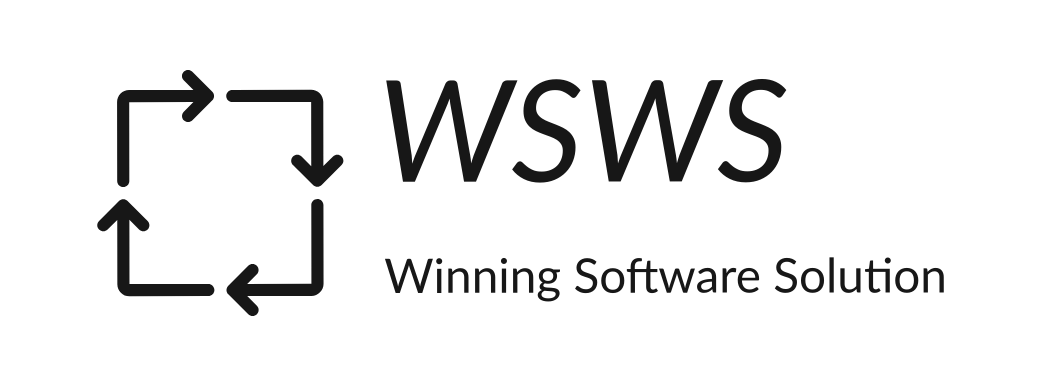
\includegraphics[width=0.4\textwidth]{../../template/WSWS-logos_transparent_crop}\\

		{\Large Winning Software Solution}\\[6pt]
		\href{mailto://winningsoftwaresolution@gmail.com}{winningsoftwaresolution@gmail.com}\\
		
		\ifdefined\progetto
		\vspace{1cm}
		{\Large\progetto}
		{\large\committenti}
		\else\fi
		
		\vspace{1.5cm}
		{\LARGE\titolo}
		
		\vfill
		
		\begin{tabular}{r | l}
		\multicolumn{2}{c}{\textit{Informazioni}}\\
		\hline
		
		\ifdefined\redattori
			\textit{Redattori} &
			\makecell[l]{\redattori}\\
		\else\fi
		\ifdefined\revisori
			\textit{Revisori} &
			\makecell[l]{\revisori}\\
		\else\fi
		\ifdefined\responsabili
			\textit{Respondabili} &
			\makecell[l]{\responsabili}\\
		\else\fi
		
		\ifdefined\versione
			\textit{Versione} & \versione
		\else\fi
		
		\textit{Uso} & \uso
		
		\end{tabular}
		
		\vspace{2cm}
		
		\ifdefined\descrizione
		Descrizione
		\vspace{6pt}
		\hrule
		\descrizione
		\else\fi
		\end{center}
	\end{titlepage}
}
\usepackage{hyperref}
\usepackage{array}
\usepackage{tabularx}

\def\vers#1-#2-#3-#4-#5\\{#1&#2&#3&#4&#5\\\hline}

\newcommand{\addversione}[5]{
	\ifdefined\versioni
		\let\old\versioni
		\renewcommand{\versioni}{#1&#2&#3&#4&#5\\\hline\old}
	\else
		\newcommand{\versioni}{#1&#2&#3&#4&#5\\\hline}
	\fi
}

\newcommand{\setversioni}[1]{\newcommand{\versioni}{#1}}

\newcommand{\makeversioni}{
	\begin{center}
		\begin{tabularx}{\textwidth}{|c|c|c|c|X|}
		\hline
		\textbf{Versione} & \textbf{Data} & \textbf{Persona} & \textbf{Attivtà} & \textbf{Descrizione} \\
		\hline
		\versioni
		\end{tabularx}
	\end{center}
	\clearpage
}

\usepackage[table,xcdraw]{xcolor}

\settitolo{Analisi delle tecnologie}
\setredattori{Federico Marchi \\ Matteo Galvagni}
\setrevisori{Giovanni Cocco}
\setdestuso{Esterno}
\setdescrizione{
Analisi delle tecnologie.
}

\addversione{0.0.0}{24/12/2021}{Matteo Galvagni}{Redazione}{Stesura iniziale sezione Introduzione e Blockchain.}
\addversione{0.0.1}{28/12/2021}{Federico Marchi}{Redazione}{Stesura iniziale sezione Backend, Pagamento e Database.}
\addversione{0.0.2}{05/01/2022}{Matteo Galvagni}{Redazione}{Stesura iniziale sezione Scansione QR code.}
\addversione{0.0.3}{10/02/2022}{Matteo Galvagni}{Redazione}{Aggiornamento di alcune tecnologie.}
\addversione{0.0.4}{11/02/2022}{Marchi Federico}{Redazione}{Correzione indice di Gulpease.}
\begin{document}

\makefrontpage

\makeversioni

\section*{Introduzione}
L'infrastruttura designata per il progetto verte sulla comunicazione diretta tra attori e blockchain. Bisognerà dunque sviluppare:
\begin{itemize}
\item un contratto digitale per lo smistamento dei fondi;
\item una landing page per facilitare il pagamento;
\item un servizio di visualizzazione di transazioni per venditori e clienti;
\item uno script per automatizzare la messa in vendita;
\item un server per fornire le pagine di consultazione e landing page;
\item un database per memorizzare gli ID delle transazioni;
\item una web app per il cliente finale per lo sblocco dei fondi e relativo controllo.
\end{itemize}
Per richiamare funzioni nel contratto sarà necessario utilizzare più librerie. Grazie a queste sarà possibile richiamare le funzioni sia lato server che lato client.

\section*{Blockchain}
La blockchain sulla quale sviluppare il contratto digitale dovrà garantire alcuni requisiti; tra questi:
\begin{itemize}
\item una elevata velocità di transazione;
\item un costo di transazione quanto più basso possibile;
\item un buon livello di sicurezza.
\end{itemize}
Questi requisiti sono richiesti al fine di garantire un buona usabilità per tutti gli attori.
Sarà inoltre cruciale la velocità e il costo ridotto per lo sblocco dei fondi.
Diverse blockchain sono state prese in esame, ma la scelta è ricaduta su Polygon; infatti:
\begin{itemize}
\item i costi di transazione sono molto bassi;
\item la velocità di transazione è ottima;
\item eredita parte delle sicurezza di Ethereum grazie al meccanismo di salvataggio a "checkpoint".
\end{itemize}
Polygon è compatibile con la Ethereum Virtual Machine. Il suo linguaggio nativo è Solidity. La documentazione esistente per questo linguaggio è esaustiva e facilmente reperibile. Verrà utilizzata la comoda e gratuita testnet di Polygon "Mumbai" per lo sviluppo del contratto.

\section*{Backend}
Sono state valutate diverse opzioni per la scelta del framework e del linguaggio per lo sviluppo lato backend. Tra questi sono stati considerati Java e Javascript; infatti ci consentono di utilizzare le librerie Web3j e Web3js. Queste librerie permettono di emettere transazioni in blockchain; inoltre permettono la comoda gestione di oggetti (transazione, contratto, ecc).
La scelta del framework è ricaduta su NodeJS e sul linguaggio Typescript; infatti ci consente di usufruire della comodità di Javascript integrando la tipizzazione; Per l'ascolto degli eventi emessi lato contratto sarà necessario un nodo presso il quale "ascoltare". La scelta è ricaduta sul servizio di API per Polygon "Moralis.io"; infatti è uno dei pochi nodi che offre un punto di accesso WebSocket e non solamente in HTTPS. Questo sarà necessario per la "sottoscrizione" ad eventi in JS.

\section*{Pagamento automatizzato alla messa in vendita}
Per automatizzare il pagamento di un oggetto con ShopChain sarà necessario integrare uno script. In particolare durante la fase di vendita. Questo script dovrà dialogare con la blockchain per creare un'istanza per il pagamento; verrà poi generato un ID univoco. Inoltre dovrà essere conservato il prezzo; infatti dovrà essere poi confrontato con il denaro inviato dal cliente all'acquisto.
Tale script verrà sviluppato in Python; permette infatti comodità di sviluppo e facilità di integrazione. Sarà necessario utilizzare la libreria "Web3py". Non utilizzando Metamask, il nodo presso la quale emettere le transazioni sarà fornito dal servizio di API per Polygon "Moralis.io".

\section*{Database}
Per la memorizzazione dei dati sulle transazioni è necessario l'utilizzo di un database. La scelta è ricaduta su MariaDB; infatti:
\begin{itemize}
\item il gruppo lo ha già utilizzato;
\item Postgres è stato escluso poiché richiede un downgrade di alcuni pacchetti Python;
\item non sono emerse necessità particolari per l'utilizzo di un database specifico.
\end{itemize}

\section*{Scansione QR code}
Il wallet Metamask su mobile non fornisce un'estensione per browser; infatti si tratta di un' applicazione con relativo browser integrato. Verrà dunque sviluppata una webapp per lo scansionamento del QR code; tale webapp dovrà permettere un comodo accesso dal browser di Metamask.

\end{document}
